\documentclass[12pt]{article}

% French
\usepackage[utf8]{inputenc}
\usepackage[T1]{fontenc}
\usepackage[french]{babel}

\usepackage{hyperref}
\usepackage{pdfpages}
\usepackage{float}
\usepackage{geometry}
\usepackage{tikz}
\usepackage{eurosym}

\usepackage{multirow}
\usepackage{datetime}

\usepackage{titlesec}

\titleformat*{\section}{\LARGE\bfseries}
\titleformat*{\subsection}{\Large\bfseries}
\titleformat*{\subsubsection}{\large\bfseries}
\titleformat*{\paragraph}{\large\bfseries}
\titleformat*{\subparagraph}{\large\bfseries}

\geometry{margin=3cm}

\definecolor{darkgreen}{RGB}{0,130,0}
\definecolor{darkblue}{RGB}{0,0,130}

\newcommand{\gameName}{\textit{Lands of Azerith}}
\newcommand{\companyName}{Stonks Industries}

\title{
    Rapport de la seconde soutenance \\
    \textbf{\gameName} \\
    \vspace{0.5cm}
    
\includegraphics[width=5cm]{assets/logo.png}
    \vspace{4.2cm}
}
\author{
    Ayemane Bouarbi \\
    \texttt{ayemane.bouarbi@epita.fr}
    \vspace{0.5cm}\and
    Louise Fussien \\
    \texttt{louise.fussien@epita.fr}
    \vspace{0.5cm}\and
    Michaël Museux \\
    \texttt{michael.museux@epita.fr}
    \vspace{0.5cm}\and
    Martin Pasquier \\
    \texttt{martin.pasquier@epita.fr}
}

\date{
    \vspace{1.5cm}
    \textbf{\companyName} \\
    \vspace{0.3cm}
    \textbf{EPITA} \\
    \vspace{1.5cm}
    \today
}

\begin{document}

\begin{titlepage}
    \maketitle
    \thispagestyle{empty} % Remove page number from title page
\end{titlepage}

\newpage
\thispagestyle{empty}
\mbox{}

\newpage
\tableofcontents


\newpage
\section{Introduction}
% Written by Louise Fussien

% This file CAN NOT be compiled on its own
% It is included by ../Book_of_Specifications.tex

\subsection{Objectif de la soutenance et du projet}

Dans le cadre de notre formation à EPITA, nous avons entrepris un projet ambitieux visant à développer un jeu vidéo. 
Ce projet, qui s'étend sur l'ensemble de l'année académique, nous a permis d'acquérir et de perfectionner nos compétences en programmation, en design de jeux et en gestion de projet. La soutenance de fin d'année marque l'aboutissement de nos efforts collectifs et individuels. 
Elle offre une occasion privilégiée de présenter l'évolution du projet, les défis surmontés et les résultats obtenus. 
\\

\subsection{Synopsis du jeu}

Lands of Azerith est un jeu d'aventure immersif où le joueur incarne un héros cherchant à libérer les terres d'Azerith de l'emprise tyrannique d'un empire dictatorial. 
L'histoire principale se déroule en trois actes, mais pour l'instant, nous nous concentrerons uniquement sur l'acte 1, qui est le seul développé et forme la base du jeu. 
Voici une description détaillée de l'acte 1, avec tous ses éléments, mécaniques et quêtes :

\subsection*{Partie 1 : Introduction et Tutoriel (Emberwood)}

L'acte 1 commence dans le village pittoresque d'Emberwood, une petite communauté nichée au milieu des ruines celtiques. Ce village sert de point de départ pour le joueur et est conçu comme une zone de tutoriel où le joueur peut se familiariser avec les différentes mécaniques du jeu. Voici les éléments clés de cette première partie :
\\

 -Choix de la Classe de Personnage : Le joueur peut choisir parmi 9 classes différentes, chacune avec ses propres compétences et styles de jeu. Les classes comprennent des guerriers, des mages, des archers, et d'autres archétypes classiques, offrant une variété de choix stratégiques. 
  \\

  \textbf{Apprentissage des Mécaniques du Jeu : }
  \\

  - Maniement des Armes : Le joueur apprend à manier différentes armes comme les haches, épées, et arcs. Chaque arme a ses propres avantages et inconvénients, et le choix de l'arme dépend de la classe choisie. 
\\

  - Équipements par Classe : Le joueur découvre les différents types d'armures (lourdes, légères) adaptées à chaque classe, influençant la mobilité et la protection. 
\\

  - Éléments : Le jeu introduit les éléments (feu, eau, vent), chacun ayant des effets spécifiques en combat et sur l'environnement. 
\\

  - Consommables : Le joueur apprend à utiliser des potions de régénération, de défense, et d'autres consommables pour survivre et se renforcer. 
\\

  - Commerce en Ville : Interactions avec les forgerons, marchands, et autres commerçants pour acheter et améliorer l'équipement. 
\\

  -  Mouvements du Personnage : Le joueur apprend à se déplacer, sauter, courir, et interagir avec l'environnement. 
  \\

-Combat Tutoriel : 

  - À la fin du tutoriel, le joueur participe à un combat d'entraînement où il met en pratique la gestion des mouvements, l'utilisation des compétences, des pouvoirs élémentaires, des armes, et des consommables. Ce combat sert de test final pour les compétences acquises. 
-Lore et Contexte :

  - En plus des mécanismes de jeu, cette première partie introduit les bases du lore de Lands of Azerith, plaçant le joueur dans un monde riche en histoire et en mystères à découvrir. 



Partie 2 : Champignome Forest 
\\
 

Après le tutoriel, le joueur est téléporté à Champignome Forest à la suite d'une défaite obligatoire à Emberwood. Cette défaite fait partie intégrante du scénario et prépare le joueur à l'intrigue principale. 

  

- Exploration de Champignome Forest : 

 La forêt est un biome mystérieux et magique, rempli de champignons géants et de créatures étranges. Le joueur doit naviguer à travers cette forêt, en utilisant les compétences apprises à Emberwood. 
\\
 
  

- Rencontre avec les Smurfcats : 

- Les Smurfcats sont des créatures amicales et importantes pour l'histoire de Champignome Forest. Ces petits chats bleus marchant sur deux pattes avec un champignon en guise de chapeau aident le joueur et introduisent la mécanique des quêtes secondaires. 

  - Quêtes Secondaires : Le joueur peut choisir d'aider les Smurfcats, ce qui offre des récompenses sous forme d'équipement bonus et influence la fin du jeu. Ces quêtes secondaires ajoutent de la profondeur à l'histoire et permettent au joueur d'explorer davantage le lore et les mystères de la forêt. 
  \\
 
 

- Objectif Principal : 

 Le joueur doit se diriger vers Gravity Crater, en passant par l'Ancient City pour récupérer un brouillard quantique calibré. Ce brouillard est une formation paranormale cruciale dans le lore du jeu et est la clé pour retourner à Emberwood. 
 \\
 

 

Suite de l'Acte 1 
\\
 

  

De retour à Emberwood, le joueur se voit refuser l'entrée et doit se rendre à Ruined Runes. Cette partie de l'acte 1 introduit de nouveaux défis et prépare le joueur pour le premier grand donjon du jeu. 
\\
 

  

- Ruined Runes et Rune Cave : 
\\
 

  - Le joueur explore Ruined Runes, une zone pleine de dangers et de mystères, avant de pénétrer dans Rune Cave, le premier donjon majeur. 
  \\
 

  - Premier Boss : A.F.I.T. (Algorithme Fabricateur à Intervalle Tertiaire) :** A.F.I.T. est une machine ancienne maîtrisant l'élément mécanique, et le joueur doit utiliser toutes les compétences et stratégies apprises pour le vaincre. Ce combat de boss enseigne les mécaniques des combats de boss, déjà introduites partiellement lors du tutoriel. 
  \\
 

  - Victoire et Récompense : Après avoir vaincu A.F.I.T., le joueur obtient un parchemin crucial pour la suite de l'histoire, qui déverrouille de nouvelles quêtes et zones. 
  \\
 

  

- Traversée de la Black Forest et du White Volcano : 
\\
 

  - Le joueur traverse la Black Forest, une zone sombre et dangereuse, puis le White Volcano, une région enneigée avec ses propres défis. Ces zones contiennent des quêtes secondaires qui permettent de récupérer plus d'équipement et d'informations sur le lore. 
  \\
 

  - Quêtes Secondaires et Lore : En explorant ces zones, le joueur découvre des notes et dialogues enrichissant l'histoire et le contexte du jeu. 
  \\
 
 

- Arrivée au King's Palace : 

 L'acte 1 se termine lorsque le joueur atteint le King's Palace, prêt à lancer l'acte 2. Ce lieu marque une étape importante dans l'histoire, offrant une transition vers de nouveaux défis et explorations. 
 \\
 

  

Progression et Lore 
\\
 

  

- Système de Quêtes : 
\\
 

  - La progression dans Lands of Azerith se fait via un système de quêtes principales et secondaires. Les quêtes principales font avancer l'histoire, tandis que les quêtes secondaires offrent des opportunités d'exploration et de personnalisation supplémentaires. 
  \\
 

  - Récompenses de Quêtes : Chaque quête accomplie offre des récompenses telles que des bonus d'expérience, de l'équipement, des consommables ou des objets spéciaux. Ces récompenses sont souvent nécessaires pour progresser dans d'autres quêtes. 
  \\
 

  

- Découverte du Lore : 
\\
 

  Le joueur en apprend davantage sur le lore du jeu en accomplissant des quêtes secondaires, en discutant avec des personnages et en collectant des notes disséminées sur la carte. Ces notes sont automatiquement stockées dans un carnet accessible à tout moment, permettant au joueur de suivre les détails de l'histoire. 
  \\
 

  

Résumé des Zones et Biomes 
\\
 

  

Lands of Azerith comprend 21 zones distinctes, chacune jouant un rôle crucial dans la progression de l'histoire et les quêtes. Voici un résumé des zones clés de l'acte 1 : 
\\
 
  

- Emberwood : Départ et tutoriel, introduction des mécanismes de jeu et du lore. 
\\
 

- Champignome Forest : Exploration et introduction aux quêtes secondaires avec les Smurfcats. 
\\
 

- Ruined Runes et Rune Cave : Premier donjon et boss, enseignement des mécaniques de combat de boss. 
\\
 

- Black Forest et White Volcano : Traversée pour atteindre le King's Palace, avec des quêtes secondaires et une exploration du lore. 
\\
 

 


\subsection{Changements depuis la dernière soutenance}

Depuis la dernière soutenance, plusieurs changements significatifs ont eu lieu au sein de notre équipe et dans le développement du projet. 
Tout d'abord, nous avons dû faire face au départ d'Alexandre Colsch, qui a quitté EPITA  pour des raisons personnelles. 
Ce départ a été compensé par l'arrivée de Louise Fussien, dont les compétences en programmation et design ont été précieuses pour la progression du projet.
\\

Ce changement fait suite à une autre transition importante : Mohamed Aziz ben Amor, un membre clé de l'équipe, était parti juste avant notre première soutenance. 
La dynamique de notre équipe a donc été profondément impactée, nécessitant une adaptation rapide et une redistribution des responsabilités.
\\

Malgré ces bouleversements, nous avons réussi à maintenir un rythme de travail soutenu et à progresser de manière significative.
\\

\subsection{Annonce de plan}

Dans ce cahier des charges, nous allons vous présenter un compte rendu détaillé de l'avancement de notre projet, en décrivant les différentes étapes de son développement, les obstacles rencontrés et les solutions mises en place. Nous aborderons également les aspects organisationnels et techniques qui ont structuré notre travail.
\newline

Tout d'abord, nous discuterons des deadlines et de l'organisation. Nous commencerons par une analyse des objectifs initiaux et des progrès réalisés jusqu'à présent. Ensuite, nous ferons un point sur l'état actuel du projet. Nous expliquerons également les délais que nous avons rencontrés et les raisons pour lesquelles ils ont été nécessaires.
\\

Ensuite, nous examinerons l'organisation du groupe. Nous décrirons les méthodes de communication utilisées au sein de l'équipe pour garantir une collaboration efficace. Nous présenterons également la répartition des tâches entre les différents membres de l'équipe, et comment nous avons utilisé GitHub pour la gestion du code source et le versionnage.
\\

Nous aborderons ensuite le nouveau cahier technique, où nous fournirons une description détaillée des aspects techniques du projet. Cela inclura des sections spécifiques sur les différents modules et composants que nous avons développés.
\\

Pour le design, nous partagerons nos sources d'inspiration et expliquerons le processus de création et d'implémentation de l'interface et de l'expérience utilisateur. Nous traiterons également de l'intégration du son et d'autres éléments multimédias.
\\

Enfin, nous discuterons du site web du projet. Nous expliquerons l'objectif du site web, son développement et son apparence finale.
\\

La conclusion fournira un récapitulatif de tout ce que nous avons accompli, ainsi que des remerciements aux personnes et aux ressources qui nous ont soutenus tout au long de ce projet.
\\

Nous inclurons également des annexes pour fournir des informations supplémentaires et les documents pertinents pour une compréhension complète du projet.
\\

Ce document vise à fournir une vue d'ensemble complète et détaillée de notre travail, en mettant en lumière notre méthodologie, nos défis, et les solutions que nous avons trouvées pour les surmonter.


\newpage
\section{Gestion des échéances et organisations}
\subsection{Analyse et progrès}

\subsubsection{Status actuel}

Depuis le début de notre projet, nous avons effectué une analyse approfondie de nos objectifs et des tâches à accomplir. L'acte un a été entièrement créé avec succès, ce qui représente une étape majeure dans l'avancement de notre projet.  

\subsubsection{Délais rencontrés et raisons}

Toutefois, notre progression a été marquée par des défis imprévus. Deux membres clés de notre équipe ont quitté le projet, ce qui a significativement impacté notre capacité de travail. Bien que l'administration ait ajouté un nouveau membre à notre groupe, cela n'a pas suffi à compenser entièrement la perte de compétences et d'expérience des membres sortants. 
\\
 

Les délais que nous avons rencontrés sont principalement dus à ces départs inattendus. L'intégration du nouveau membre a pris du temps, non seulement pour qu'il se familiarise avec le projet, mais aussi pour qu'il soit pleinement opérationnel. De plus, notre ambition de perfectionnisme a joué un rôle important. Nous avons été très méticuleux dans chaque étape du développement, ce qui, bien que bénéfique pour la qualité du projet, nous a obligé à raccourcir le nombre d’actes prévus initialement. 
\subsection{Organisation du groupe}

\subsubsection{Communication}

Pour assurer une collaboration efficace au sein de notre groupe de projet, nous avons opté pour l'utilisation de plusieurs outils de communication. Principalement, nous avons utilisé Discord, une plateforme de communication instantanée, pour faciliter les échanges en temps réel entre les membres du groupe. Discord nous a permis de maintenir une communication fluide et réactive, essentielle pour coordonner nos efforts et résoudre rapidement les problèmes rencontrés pendant le développement du projet. Les fonctionnalités de chat vocal et textuel de Discord ont été particulièrement utiles pour organiser des réunions spontanées et des discussions en groupe, améliorant ainsi notre efficacité collaborative. 
\\

En complément de Discord, nous avons également profité des sessions de travail en groupe en présentiel à l'EPITA. Ces rencontres physiques nous ont offert l'opportunité de discuter en profondeur des aspects techniques et conceptuels du projet, de partager des idées de manière plus interactive et de travailler sur des tâches spécifiques ensemble. Cette combinaison d'interaction en ligne via Discord et en personne à l'université nous a permis de tirer parti des avantages uniques de chaque mode de communication, 
renforçant ainsi notre cohésion d'équipe et notre efficacité dans l'accomplissement des objectifs du projet. 
\\



\subsubsection{GitHub}

Github a joué un rôle central dans la gestion et le partage de notre code source tout au long du projet. 
Nous avons utilisé GitHub comme plateforme principale pour héberger notre repository de projet, ce qui nous a permis de collaborer efficacement sur le code. 
Chaque membre du groupe a pu créer des branches de développement distinctes pour travailler sur des fonctionnalités spécifiques sans perturber la branche principale, tout en utilisant des pull requests pour fusionner les contributions et effectuer des révisions par les pairs.
\\

L'intégration de GitHub avec notre flux de travail nous a offert plusieurs avantages. 
Premièrement, cela a facilité la gestion des versions du code et le suivi des modifications apportées à mesure que le projet évoluait. 
Deuxièmement, GitHub a facilité la détection et la résolution des conflits de fusion, assurant ainsi l'intégrité du code source partagé entre les membres du groupe. 
\\
\subsubsection{Répartition des tâches }


La répartition des charges au sein de notre équipe a été stratégique et s'est adaptée aux défis que nous avons rencontrés tout au long du projet.
 Initialement, chaque membre de l'équipe s'est vu attribuer des responsabilités spécifiques en fonction de ses compétences et de son expertise, 
 telles que définies dans le cahier des charges technique initial.
\\ 

Cependant, notre progression a été marquée par des changements significatifs. 
Nous avons dû faire face au départ inattendu de deux membres clés de l'équipe. 
Cela a eu un impact direct sur notre capacité à respecter les délais et à maintenir la cohésion au sein du groupe. Pour pallier ces départs, sans recruter de nouvelles personnes, l'administration a intégré un nouveau membre existant dans notre groupe.
\\

Cette transition n'a pas été sans défis. L'intégration du nouveau membre a demandé du temps pour s'adapter aux dynamiques de l'équipe et pour assimiler les responsabilités en cours. Malgré ces ajustements, nous avons maintenu une communication ouverte et des réunions régulières pour aligner les attentes et assurer une collaboration harmonieuse.
\\

Au fur et à mesure que nous nous sommes adaptés à ces changements, 
nous avons également mis à jour notre cahier des charges technique pour refléter les nouvelles répartitions et les ajustements nécessaires. 
Chaque nouvelle itération du cahier technique a intégré les modifications stratégiques et les décisions prises en réponse aux défis rencontrés,
 y compris la redistribution des tâches et des responsabilités entre les membres existants.
\\

\subsubsection{Cahier des charges techniques}
Pendant le développement du projet, nous avons élaboré plusieurs versions du cahier technique pour répondre aux évolutions et aux défis rencontrés. Chaque itération a été cruciale pour ajuster notre approche et nos spécifications en fonction des besoins changeants du projet. 
\\

Initialement, notre cahier technique définissait les fondations et les objectifs techniques de notre jeu. Nous avons spécifié les fonctionnalités essentielles, l'architecture logicielle prévue, ainsi que les technologies clés à utiliser. Cette première version nous a permis de commencer le développement sur des bases solides. 
\\

 


Le dernier cahier des charges technique, intégré dans ce rapport final, reflète ces ajustements. Il décrit non seulement les spécifications finales du jeu telles qu'elles ont évolué tout au long du processus, mais aussi les décisions stratégiques prises pour surmonter les défis rencontrés. 

\newpage
\section{Partie technique}
% Written by Louise Fussien

% This file CAN NOT be compiled on its own
% It is included by ../Book_of_Specifications.tex


\subsection{Environnement de travail}


\subsection*{Introduction à l'Environnement de Travail}
Dans le cadre de notre projet, nous avons choisi d'utiliser le moteur de jeu Godot en conjonction avec l'environnement de développement intégré (IDE) Rider.
 Cette configuration a été sélectionnée pour ses capacités avancées en matière de développement de jeux vidéo, ainsi que pour la flexibilité et les outils de 
 débogage puissants offerts par Rider.

 \subsection*{Fonctionnement de Godot et Intégration avec Rider}
\textbf{Godot} est un moteur de jeu open-source, reconnu pour sa facilité d'utilisation et sa capacité à 
gérer des projets de jeux vidéo en 2D et en 3D. Il offre une gamme complète de fonctionnalités, y compris un éditeur visuel intuitif,
 des systèmes de scripting flexibles grâce à GDScript (un langage de script similaire à Python), ou C\# et des outils robustes pour l'animation 
 et la physique. Le choix de Godot a été motivé par sa communauté active et ses ressources abondantes, facilitant ainsi l'apprentissage et la résolution de problèmes.
\\

 \textbf{Rider}, développé par JetBrains, est un IDE multiplateforme qui offre un support étendu pour de nombreux langages de programmation, notamment C\#. Son
  intégration avec Godot permet d'exploiter pleinement les capacités de scripting C\# de Godot, offrant ainsi une expérience de développement plus enrichissante et productive. Rider propose également des outils de refactoring, une navigation améliorée dans le code, et des capacités de débogage avancées, qui sont particulièrement utiles pour les projets complexes de jeux vidéo.

\subsection*{Défis Associés aux Changements de Version de Godot}
L'un des défis majeurs rencontrés dans notre environnement de travail est lié aux changements de version de Godot. Le moteur est en constante évolution, 
avec des mises à jour fréquentes qui apportent de nouvelles fonctionnalités et des améliorations de performance. Cependant, ces mises à jour peuvent 
également introduire des modifications significatives qui affectent la compatibilité du code existant.
\\

Pour une partie de notre groupe, moins expérimentée dans la conception de jeux vidéo, ces changements de version ont posé des problèmes d'adaptation.
 Les différences entre les versions peuvent inclure des modifications dans l'API, des changements de comportement dans les outils d'animation ou de physique, 
 et des ajustements dans les méthodes de rendu graphique. Ces modifications nécessitent une compréhension approfondie des nouvelles fonctionnalités et des 
 ajustements potentiellement complexes du code existant pour maintenir la stabilité et les performances du projet.
\\

Afin de surmonter ces défis, nous avons mis en place plusieurs stratégies :
\\

-Documentation et Formation : Nous avons organisé des sessions de formation interne pour familiariser l'équipe avec les nouvelles fonctionnalités 
et les changements apportés par les mises à jour de Godot. Des tutoriels et des guides spécifiques ont été créés pour faciliter l'apprentissage.
\\


-Environnement de Test : Avant de migrer vers une nouvelle version de Godot, nous avons établi un environnement de test dédié pour évaluer l'impact 
des changements sur notre projet. Cela nous permet de repérer et de corriger les incompatibilités potentielles avant d'intégrer les modifications dans la branche principale du projet.
\\

-Révision de Code et Pair Programming : Nous avons encouragé la révision de code et le pair programming, où des membres plus expérimentés de l'équipe 
travaillent en étroite collaboration avec ceux moins expérimentés, pour partager des connaissances et assurer une transition en douceur entre les versions.

\subsection{Manipulation des Fichiers JSON : Défis et Solutions}

\subsection*{Introduction à JSON et son Utilisation dans le Développement de Jeux}
JavaScript Object Notation (JSON) est un format de données léger et facile à lire et écrire pour les humains, et facile à analyser et générer pour les machines. 
JSON est largement utilisé dans le développement de jeux vidéo pour stocker et échanger des données structurées. Dans notre projet, nous avons utilisé des fichiers 
JSON pour stocker divers éléments du jeu, y compris des images de texte, des configurations de jeu, et des données de sauvegarde.
\\

\subsection*{Compréhension et Manipulation des Fichiers JSON}
Lors de notre première tentative d'intégration de fichiers JSON dans notre projet de jeu vidéo, nous avons 
rencontré plusieurs difficultés en raison de notre manque initial de familiarité avec ce format de fichier. Pour remédier à cela, 
nous avons entrepris une étude approfondie de JSON et de ses applications dans le contexte de notre projet.

\subsection*{Structure et Syntaxe de JSON}
JSON représente des données sous forme de paires clé/valeur et de tableaux. Une paire clé/valeur se compose d'un nom de champ (clé) et de sa valeur associée. 
Les valeurs peuvent être des chaînes de caractères, des nombres, des objets (des paires clé/valeur imbriquées), des tableaux, des booléens (true/false), ou null.
\\

Exemple de structure JSON : 

\begin{figure}[H]
      \centering
      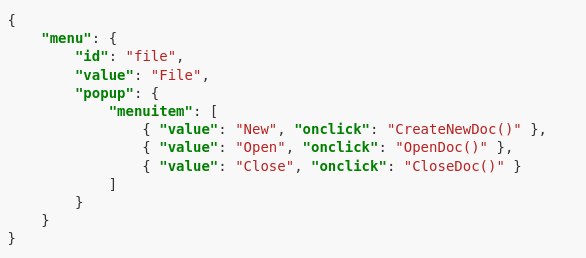
\includegraphics[width=0.8\textwidth]{assets/jsonexemple.png}
      
      \label{fig:json}
  \end{figure}

L'intégration de fichiers JSON dans notre code s'est révélée être un défi considérable mais stimulant. 
Voici un aperçu détaillé du processus et des solutions mises en œuvre pour surmonter les obstacles techniques :
\\

\textbf{1-Lecture et Écriture de Fichiers JSON :}
La première étape consistait à lire les données à partir des fichiers JSON et à les écrire dans ces fichiers. 
Nous avons utilisé les bibliothèques de gestion des fichiers JSON disponibles dans les langages de programmation utilisés dans notre projet.
 En C\#, par exemple, nous avons exploité les classes JsonSerializer et JsonDeserializer fournies par le framework .NET.
\\

\textbf{2-Sélection des Attributs à Sauvegarder :}
Une des tâches cruciales était de déterminer quels attributs des objets de jeu devaient être sauvegardés dans les fichiers JSON. Pour cela, 
nous avons effectué une analyse approfondie des besoins du jeu et de la pertinence des données à long terme. Les attributs essentiels comme les
statistiques des personnages, l'état de l'inventaire, et les positions des objets dans le monde de jeu ont été jugés importants. En revanche, 
les attributs temporaires ou dérivables, comme les états intermédiaires de certaines animations, ont été exclus pour éviter un gonflement inutile des fichiers de sauvegarde.
\\

\textbf{3-Récupération des Objets à Partir de Fichiers JSON :}
Une fois les fichiers JSON créés, la prochaine étape consistait à récupérer les objets de jeu à partir de ces fichiers. 
Ce processus impliquait de désérialiser les données JSON en objets utilisables dans notre moteur de jeu. 
L'un des défis majeurs ici était de garantir que les données récupérées soient correctement mappées aux structures de
données de notre jeu, en respectant les types et les contraintes de chaque attribut.


\subsection{L'architecture du jeu}




L'architecture d'un projet de développement de jeux vidéo est essentielle pour assurer une organisation claire et une gestion efficace des ressources.
 Dans notre projet, nous avons adopté une structure de dossiers bien définie pour faciliter la gestion des différents composants du jeu. Cette organisation 
 a permis de simplifier le processus de développement, de faciliter la collaboration entre les membres de l'équipe et d'assurer une maintenance efficace du code
  et des ressources. Voici une description détaillée de la structure de notre projet et du rôle de chaque dossier.

\subsection*{Structure des Dossiers}

1. Dossier Assets

   Le dossier `assets` est le répertoire principal qui contient toutes les ressources visuelles et sonores utilisées dans le jeu. 
   Ce dossier est crucial pour centraliser toutes les images, les sons, les textures et autres médias nécessaires pour le développement du jeu.

   - Contenu : Images, textures, sons, et autres médias.

   - Exemple : `assets/background.png`, `assets/music/theme.mp3`.
\\

2. Dossier Caractères

   Le dossier `caractères` est dédié aux images des personnages du jeu, incluant à la fois le joueur et les monstres.
    Cette séparation permet une gestion plus facile et une localisation rapide des ressources graphiques liées aux entités interactives du jeu.
   
   - Contenu : Images des personnages joueurs et des monstres.
  
   - Exemple : `caractères/joueur.png`, `caractères/monstre.png`.
\\

3. Dossier Items

   Le dossier `items` contient les fichiers JSON associés aux différents objets (items) présents dans le jeu. 
   Ces fichiers JSON définissent les attributs et les propriétés des objets, tels que leur nom, description, valeur, et effets en jeu.

   - Contenu : Fichiers JSON des objets.

   - Exemple : `items/potion.json`, `items/épée.json`.
\\

4. Dossier Loottables

   Le dossier `loottables` est associé aux données d'objets donnés par la mort des monstres. 
   Ces fichiers permettent de générer les objets qui seront donnés par les monstres à leur mort.

   - Contenu : Fichiers JSON pour les objets des monstres.
\\

5. Dossier Mob

   Le dossier `mob` contient les fichiers JSON des monstres, décrivant leurs caractéristiques, comportements et statistiques. Ces fichiers jouent un rôle crucial dans la définition des ennemis que les joueurs rencontreront dans le jeu.

   - Contenu : Fichiers JSON des monstres.

   - Exemple : `mob/zombie.json`, `mob/dragon.json`.
   \\

6. Dossier Quest

   Le dossier `quest` contient les fichiers JSON associés aux quêtes du jeu. Chaque fichier JSON représente une quête, incluant des informations telles que les objectifs, les récompenses, et les dialogues associés.

   - Contenu : Fichiers JSON des quêtes.

   - Exemple : `quest/quête1.json`, `quest/quête2.json`.
\\

7. Dossier Scenes

   Le dossier `scenes` contient toutes les scènes utilisées dans le moteur Godot. Une scène dans Godot représente une collection d'objets (nodes) organisés de manière hiérarchique. Ce dossier est essentiel pour structurer les différents niveaux et interfaces du jeu.

   - Contenu : Fichiers de scènes Godot.

   - Exemple : `scenes/menu.tscn`, `scenes/niveau1.tscn`.
\\

8. Dossier Script

   Le dossier `script` contient tous les scripts utilisés dans le projet. Ces scripts sont écrits en C\#, et sont responsables de la logique de jeu, des interactions des personnages, et des comportements des objets.

   - Contenu : Scripts de jeu.


      \subsection{Menu du Jeu }

      % inserer image du menu

      \subsubsection*{Introduction à l'Effet Parallax dans le Menu}
      L'effet parallax est une technique visuelle utilisée pour créer une sensation de profondeur en animant différents plans à des vitesses différentes.
      Dans notre jeu, nous avons implémenté un effet parallax dans le menu principal pour donner une impression de perspective en 2D. 
      Voici comment nous avons structuré et mis en œuvre cet effet de manière efficace et immersive.
      \\

      \subsubsection*{Implémentation de l'Effet Parallax}
      Nous avons créé une node principale ParallaxBackground dans Godot, qui agit comme le conteneur global pour notre effet parallax.
      Cette node a des enfants (fils) correspondant à chaque plan de fond que nous voulons animer. Chaque plan a une image différente et une
      vitesse de défilement spécifique, ce qui crée une illusion de profondeur lorsque le joueur navigue dans le menu.
      \\

      \subsubsection*{Structure de la Node ParallaxBackground}
      La node ParallaxBackground est configurée avec plusieurs enfants (fils), chacun représentant un plan de fond distinct.
      Chaque plan est un sprite ou une texture avec une image unique et est déplacé à une vitesse différente par rapport aux autres plans pour simuler la perspective.
      \\

      Exemple de structure de la node ParallaxBackground :
      \\

      \begin{figure}[H]
            \centering
            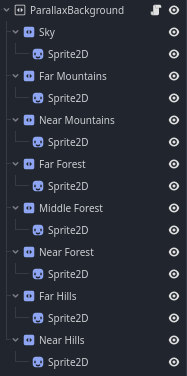
\includegraphics[width=0.3\textwidth]{assets/paralax.png}
            
            \label{fig:website1}
        \end{figure}

      \subsubsection*{Animation et Effet Visuel}
      Chaque plan de fond est animé en ajustant sa position horizontale à chaque trame (frame) du jeu, en fonction de sa vitesse définie.
      Les plans plus proches (vitesse plus faible) se déplacent plus lentement par rapport à ceux qui sont plus éloignés (vitesse plus élevée), 
      créant ainsi un effet de parallaxe réaliste qui renforce l'immersion du joueur dès le lancement du jeu.
      \\
      \subsection{Le Multijoueur}

      Pour pouvoir organiser une partie multijoueur, nous avons décidé d'utiliser l'API intégrée à Godot.
      Pour cela, il nous faut un serveur, ici l'hôte, ainsi que les joueurs qui rejoignent sa partie appelés les clients,
      En premier temps, l'hôte doit appuyer sur le bouton 'Host' puis les joueurs doivent accéder à l'adresse de l'hôte, et appuyer sur le bouton 'Join'.

      Il est possible de jouer avec un nombre infini de joueurs, mais nous avons établi un maximum de 8, limite que nous utiliserons lors de la conception du reste du jeu.
      \\

      Maintenant que la connexion est établie entre les différents joueurs, il nous faut synchroniser leurs informations entre eux, 
      tout en faisant attention à ne pas trop partager d'informations inutiles, pour limiter l'utilisation de bande passante.
      Par exemple, la synchronisation des positions de chacun entre tous les joueurs est importante, 
      mais la position de la caméra d'un joueur n'est nécessaire qu'en local (c.f. Figures \ref*{fig:gameplay3} et \ref*{fig:gameplay4}).


      \subsubsection*{Système de Connexion Multi-joueurs via Envoi de Paquets}
      Pour permettre une connectivité multi-joueurs fluide et intuitive, nous avons implémenté un système de gestion de serveur 
      et de connexion basé sur l'envoi de paquets. Ce système est conçu pour simplifier l'expérience des joueurs en éliminant 
      la nécessité d'entrer manuellement les adresses IP des serveurs.

      \subsection*{Fonctionnement du Système}
      \textbf{1- Serveur d'Hébergement :}

      Lorsqu'un joueur décide d'héberger une partie, le jeu démarre un serveur local et commence à envoyer des paquets d'informations à intervalles réguliers 
      (par exemple, toutes les secondes).
      Chaque paquet contient des détails essentiels comme le nom du serveur, l'adresse IP du serveur, et le nombre actuel de joueurs connectés.
      \\

      \textbf{2-Joueurs Rejoignant le Serveur :}

      Les autres joueurs du réseau écoutent en permanence les paquets émis par les serveurs disponibles.
      Lorsqu'un paquet est détecté, les détails du serveur sont affichés à l'écran, permettant aux joueurs de visualiser facilement les serveurs disponibles ainsi que les informations pertinentes comme le nom et le nombre de joueurs.
      Un bouton "Rejoindre" est proposé aux joueurs pour se connecter au serveur sélectionné, simplifiant ainsi le processus de connexion.
\\

      \textbf{3-Démarrage de la Partie :}

      Une fois que les joueurs se sont connectés au serveur et que le nombre requis est atteint, un bouton "Start" devient accessible à tous les participants.
      Lorsque tous les joueurs ont cliqué sur "Start", la partie commence, permettant ainsi de synchroniser l'expérience de jeu pour tous les participants.

      \subsubsection*{Avantages du Système de Paquets}

      Ce système de connexion basé sur l'envoi de paquets présente plusieurs avantages :
\\

      -Simplicité d'utilisation : Les joueurs n'ont pas besoin de connaître l'adresse IP du serveur manuellement.
      \\

      -Visibilité et Accessibilité : Les informations sur les serveurs disponibles sont clairement affichées, facilitant ainsi la sélection et la connexion.
      \\

      -Synchronisation Facile : Tous les joueurs sont automatiquement informés des détails du jeu en cours, assurant ainsi une expérience de jeu fluide et harmonieuse.



      \subsection{Contrôles et Interaction dans le Jeu}

      Les contrôles et interactions jouent un rôle crucial dans l'expérience de jeu, 
      assurant une navigation fluide et intuitive à travers l'environnement virtuel. 
      Dans notre jeu développé sous Godot, nous avons mis en œuvre plusieurs fonctionnalités de contrôle permettant aux joueurs de se déplacer, 
      d'interagir avec l'environnement, de gérer leur inventaire et de lancer des actions spécifiques avec facilité.
      \\

      Les déplacements du joueur sont gérés à l'aide des touches Z, Q, S, et D, qui correspondent respectivement aux directions Haut, Gauche, Bas, et Droite sur le clavier. 
      Cette configuration permet une navigation fluide dans les différents niveaux du jeu. 
      L'utilisation de la librairie d'entrée de Godot facilite la détection des touches pressées et assure une réponse instantanée aux actions du joueur.

      \subsection*{Actions Spécifiques}
      \textbf{Quitter le Jeu avec la Touche Echap}

      Pour offrir une sortie rapide et intuitive du jeu, la touche Echap est associée à la fonction de fermeture de l'application. 
      Cela permet aux joueurs de quitter le jeu à tout moment sans effort, tout en libérant proprement toutes les ressources utilisées par le jeu.
      \\

      \textbf{Courir avec la Touche Shift}

      La touche Majuscule est utilisée pour activer le mode de course du joueur, augmentant ainsi sa vitesse de déplacement. Ce mécanisme permet aux joueurs de se déplacer plus rapidement lorsqu'ils ont besoin d'atteindre des destinations plus éloignées ou de fuir des dangers potentiels dans le jeu.
      \\

      \textbf{Ouvrir l'Inventaire avec la Touche Tab}

      L'inventaire est une composante essentielle de nombreux jeux, offrant aux joueurs la possibilité de gérer leurs objets, équipements et ressources. Dans notre jeu, l'inventaire est accessible en appuyant sur la touche Tab, facilitant ainsi la gestion des items collectés et des équipements utilisés par le joueur.
      \\

      \textbf{Attaquer avec le Clic Gauche de la Souris}

      Pour interagir avec les monstres et autres éléments interactifs dans le jeu, les joueurs peuvent utiliser le clic gauche de la souris. Ce mécanisme permet de lancer des attaques, d'activer des objets ou d'interagir avec des éléments du décor, offrant ainsi une expérience immersive et dynamique.
      \\

      \textbf{Implémentation Technique}

      Chaque fonctionnalité de contrôle est implémentée en utilisant les capacités intégrées de Godot pour gérer
      les événements d'entrée et les interactions utilisateur. Cette approche assure une cohérence dans le traitement des actions du joueur 
      et garantit une jouabilité fluide et intuitive tout au long du jeu.


      \subsection{Intelligence Artificielle : Comportements des Monstres}
      Dans notre jeu, nous avons implémenté différents comportements pour les monstres afin d'enrichir l'interaction avec le joueur. 
      Chaque type de monstre possède des caractéristiques et des réactions spécifiques, déterminées par une classe dédiée qui gère son comportement en
      fonction des interactions avec le joueur.

      \subsection*{Types de Monstres}

      Nous avons défini quatre types de monstres, chacun ayant un comportement distinct en fonction de la proximité et des actions du joueur :
      \\

      -Agressif :

      Ce type de monstre attaque activement le joueur dès qu'il est à proximité.
      Lorsque le joueur entre dans sa zone de détection, le monstre commence à se déplacer vers le joueur pour l'attaquer.
      En cas de contact avec le joueur, le monstre déclenche une attaque ou une réaction offensive.
      \\

      -Neutre :

      Les monstres neutres ne sont pas agressifs par nature mais répondent si le joueur les attaque.
      Lorsque le joueur les agresse, ils changent leur comportement pour devenir agressifs et attaquent en retour.
      En dehors des attaques contre eux, ils continuent leurs activités normales sans réaction offensive.
      \\

      -Passif :

      Les monstres passifs ne cherchent pas à attaquer le joueur et fuient s'il est agressé.
      Lorsque le joueur les attaque, ils s'éloignent activement du joueur pour éviter tout contact et toute confrontation directe.
      \\

      -Peureux :

      Les monstres peureux évitent activement tout contact avec le joueur.
      Dès que le joueur s'approche, ils tentent de s'éloigner rapidement et de fuir la zone de danger.


      \subsection*{Implémentation Technique}
      Chaque type de monstre est implémenté à l'aide de classes distinctes dans Godot, 
      chacune étant responsable de la gestion des comportements spécifiques décrits ci-dessus.
      Voici comment nous avons mis en œuvre ces comportements complexes à l'aide des capacités de détection de collisions et de signaux de Godot :
      \\

      \textbf{Détection de Collision avec CollisionShape2D}

      Chaque monstre est équipé d'une CollisionShape2D dans Godot, configurée pour détecter les collisions avec le joueur et d'autres entités du jeu. 
      Cette forme de collision est essentielle pour déclencher des actions basées sur la proximité et les interactions spatiales avec d'autres nodes dans la scène.
      \\

      \textbf{Utilisation de Area2D pour les Signaux}

      Nous utilisons également des nodes Area2D pour émettre des signaux vers la node principale du monstre.
      Ces signaux sont utilisés pour détecter quand le joueur entre dans la zone de détection du monstre, 
      ce qui déclenche un changement de comportement en fonction du type de monstre :
      \\

      Pour les monstres agressifs et neutres : lorsque le joueur entre dans la zone, le monstre commence à se déplacer vers le joueur pour l'attaquer 
      (si neutre, il attaque en retour si attaqué).
      \\

      Pour les monstres passifs et peureux : lorsque le joueur entre dans la zone, le monstre s'éloigne activement du joueur pour éviter le contact.
      \\

      \textbf{Gestion des Comportements Dynamiques}

      Chaque classe de monstre gère de manière dynamique son comportement en réponse aux signaux émis par Area2D. 


      \begin{figure}[H]
            \centering
            
\includegraphics[width=0.6\textwidth]{assets/mob.png}
            \caption{Exemple du signal émis par le mob}
            \label{fig:website1}
        \end{figure}





\subsection{Déplacement des Monstres avec Navigation A* }




Dans notre jeu, nous avons intégré des mécanismes avancés pour le déplacement des monstres en utilisant le système de navigation A* (A-star) et 
la gestion de l'inventaire du joueur. Ces fonctionnalités améliorent l'expérience de jeu en offrant des déplacements fluides et des interactions riches
 avec les objets collectés. Voici comment nous avons implémenté ces fonctionnalités techniques dans Godot.

\subsection*{Déplacement des Monstres avec Navigation A*}

Pour permettre aux monstres de se déplacer intelligemment dans l'environnement du jeu, nous avons utilisé la node 
\texttt{Navigation2D} de Godot, qui intègre un système de pathfinding basé sur l'algorithme A*. Cela permet aux monstres 
de calculer automatiquement le chemin le plus optimal vers leur cible, comme le joueur ou un point spécifique de la carte.

\subsection*{Implémentation de la Node \texttt{Navigation2D}}

La node \texttt{Navigation2D} est configurée pour représenter la carte jouable du jeu, 
avec des obstacles et des zones de passage définies. Voici comment elle est utilisée dans Godot :
\\

\begin{itemize}
    \item \textbf{Configuration de la Navigation} :
     Nous avons généré une carte de navigation en plaçant des obstacles et en définissant les zones accessibles par les monstres.
      Cette carte est utilisée par l'algorithme A* pour calculer les chemins.
    \\

    \item \textbf{Utilisation de \texttt{Navigation2D} dans le Code} : Chaque monstre 
    est doté d'une instance de \texttt{Navigation2D}, configurée pour calculer un chemin vers sa cible actuelle à intervalles réguliers.
\end{itemize}

\subsection*{Déplacement Dynamique des Monstres}

À intervalles réguliers, les monstres recalculent leur chemin vers leur cible (par exemple, le joueur) en utilisant la fonctionnalité
 de \texttt{Navigation2D}. Cela garantit que les monstres peuvent naviguer efficacement autour des obstacles et trouver le chemin le plus court pour
  atteindre leur objectif.



\subsection*{Aléatoire dans le Rayon de Déplacement}

Pour ajouter une variabilité aux déplacements des monstres, toutes les 5 secondes, chaque monstre a une chance sur trois de choisir une nouvelle
 destination aléatoire à l'intérieur d'un rayon de 300 pixels autour de sa position actuelle. Cela simule un comportement plus organique et imprévisible des monstres,
  rendant leur présence dans le jeu plus dynamique et réaliste.


\subsection*{Spawning des Monstres dans une Zone Définie}

Pour enrichir l'exploration du joueur et maintenir la dynamique du jeu, nous avons mis en place un système de spawn de monstres dans des zones prédéfinies :
\\

\begin{itemize}
    \item \textbf{Zone de Spawn Rectangulaire} : Nous avons défini une zone rectangulaire dans la carte du jeu où les monstres peuvent apparaître périodiquement.
    \\

    \item \textbf{Instantiation des Monstres} : Toutes les 15 secondes, un nouveau monstre est instancié dans cette zone de spawn si la limite de monstres dans
     cette zone n'est pas atteinte.
    \\

    \item \textbf{Chargement Dynamique depuis un Fichier JSON} : Chaque type de monstre est associé à un fichier 
    JSON qui contient ses caractéristiques, comme ses attributs, ses comportements et ses statistiques. Lorsqu'un monstre est instancié, 
    ces informations sont chargées à partir du fichier JSON correspondant.
\end{itemize}

\subsection{Gestion de l'inventaire du joueur }

\subsection*{Structure de l'Inventaire}

L'inventaire est représenté par un tableau de cases, où chaque case peut contenir un objet spécifique avec sa quantité. 
Les joueurs peuvent visualiser leur inventaire en appuyant sur la touche \texttt{Tab}, ce qui ouvre une interface utilisateur affichant 
les objets collectés et leur quantité respective.

\subsection*{Interaction avec l'Inventaire}

\begin{itemize}
    \item \textbf{Ajout d'Objets} : Lorsque le joueur ramasse un nouvel objet, celui-ci est ajouté à l'inventaire s'il n'est pas déjà présent. 
    Si l'objet est déjà présent, la quantité existante est simplement mise à jour.
    \\
    \item \textbf{Affichage et Gestion} : L'interface de l'inventaire permet aux joueurs de visualiser, utiliser et organiser leurs objets selon 
    leurs besoins. Par exemple, les objets peuvent être équipés, consommés ou échangés selon leur utilité dans le jeu.
\end{itemize}

gameN


\subsection{Gestion des Points de Vie, Checkpoints et Loot dans le Jeu}

Dans notre jeu, nous avons mis en place un système robuste pour gérer les points de vie du joueur, 
les checkpoints pour la réapparition, et la mécanique de loot des monstres. Voici comment chaque aspect 
est implémenté pour enrichir l'expérience de jeu et assurer une progression gratifiante pour les joueurs.

\section*{Points de Vie du Joueur}

Le joueur démarre avec un nombre initial de points de vie (PV) fixé à 1000. Lorsqu'il subit une attaque de la part d'un monstre ou d'un autre ennemi,
 les dégâts infligés sont calculés en fonction de la force de l'attaque et des attributs de l'arme de l'attaquant.

\subsection*{Calcul des Dégâts}

Les dégâts subis par le joueur sont calculés en fonction de la formule suivante, basée sur la force de l'attaque 
(\textit{force\_attaque}) et le nombre de points de l'arme (\textit{points\_arme}) de l'attaquant : (\textit{points\_arme}) + (\textit{force\_attaque})
\\

Cela permet d'ajuster dynamiquement les dégâts en fonction de la puissance de l'attaque et de 
l'équipement de l'attaquant, ajoutant ainsi une couche de stratégie et de gestion des ressources pour le joueur.

\section*{Gestion des Checkpoints}

Pour assurer une progression fluide et éviter une perte de progrès significative en cas de mort du joueur, nous avons intégré un système de checkpoints :
\\

\begin{itemize}
    \item \textbf{Réapparition au Dernier Checkpoint} : Lorsque le joueur meurt, il réapparaît au dernier checkpoint atteint. Cette fonctionnalité est essentielle pour réduire la frustration du joueur et encourager l'exploration sans crainte de perdre tout son progrès.
    \\

    \item \textbf{Restauration des Points de Vie Maximum} : À chaque réapparition, le joueur récupère ses points de vie maximum, lui permettant de reprendre le jeu avec une chance égale de succès.
\end{itemize}

\section*{Mécanique de Loot des Monstres}

Lorsqu'un monstre est vaincu, plusieurs actions se produisent pour enrichir l'expérience du joueur :
\\
\begin{itemize}
    \item \textbf{Loot des Objets Associés au Monstre} : Chaque type de monstre est associé à un fichier JSON définissant les objets qu'il peut lâcher lorsqu'il meurt. Ces objets peuvent inclure des équipements, des ressources ou d'autres items précieux pour la progression du joueur.
    \\

    \item \textbf{Apparition de Débris et Textures} : Pour indiquer visuellement la mort du monstre, des débris et des textures spécifiques à ce monstre apparaissent à l'emplacement où il a été vaincu. Cela crée une immersion et une satisfaction visuelle pour le joueur.
    \\

    \item \textbf{Récupération des Objets par le Joueur} : Lorsque le joueur passe sur les débris et textures laissés par le monstre, il récupère automatiquement les objets associés dans son inventaire. Cela simplifie le processus de collecte et de gestion des objets obtenus lors des combats.
\end{itemize}




\subsection{Génération de Map et Gestion des Transitions avec Nodes dans Godot}




Dans notre jeu, la création et la gestion des textures de la carte ainsi que les transitions fluides entre les différents environnements sont
 des aspects cruciaux pour offrir une expérience visuelle immersive et dynamique. Voici comment nous avons implémenté ces fonctionnalités techniques 
 avancées dans Godot, en nous concentrant sur la génération de la carte, les transitions entre les maps et l'animation des personnages et des objets.

\section*{Génération de la Map et Utilisation des Textures}

La carte du jeu est entièrement générée et dessinée par notre designer, ce qui nous permet de contrôler précisément 
l'aspect visuel et le design de chaque environnement.
 Voici comment nous avons structuré notre approche :

\subsection*{Textures et Tiles}

Pour la création de la carte, nous utilisons des textures organisées en tiles. 
Chaque tile représente une partie spécifique de la carte, telle que le sol et les éléments statiques qui ne bougent pas.
 Ces textures sont soigneusement intégrées dans la map pour former des environnements cohérents et esthétiquement plaisants.

\subsection*{Tileset pour les Maps}

Les tilesets sont des images contenant plusieurs textures utilisées pour les maps. Ils permettent de définir les décors,
 les détails du sol et d'autres éléments fixes qui ne changent pas pendant le jeu. Cela garantit une cohérence visuelle et simplifie
  la gestion des textures dans l'environnement du jeu.


  \begin{figure}[H]
      \centering
      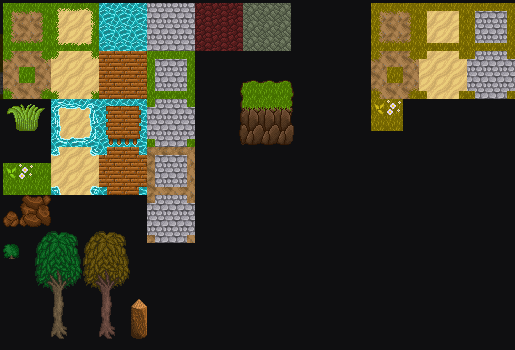
\includegraphics[width=0.8\textwidth]{assets/tileset.png}
      \caption{Nos textures}
      \label{fig:website1}
  \end{figure}

\section*{Gestion des Transitions entre les Maps}

Les transitions entre les différentes zones de la carte sont gérées à l'aide de nodes spécifiques qui assurent une expérience de jeu fluide et immersive :

\subsection*{Nodes de Transition}

Chaque zone de transition est représentée par une node comportant un \texttt{Area2D} et une \texttt{CollisionShape2D}.
 Lorsque le joueur entre dans cette zone, des événements sont déclenchés pour faire apparaître la nouvelle map, faire disparaître l'ancienne et ajuster les coordonnées du joueur, créant ainsi une illusion de téléportation fluide et réaliste.

\subsection*{Changement Dynamique de la Map}

Lorsque le joueur traverse une zone de transition, le jeu procède à un chargement dynamique de la nouvelle map tout en 
déchargeant celle précédente. Cela permet de maintenir une utilisation efficace des ressources tout en offrant une navigation sans heurts à 
travers les différentes zones de jeu.

\section*{Animation des Personnages et des Objets}

Pour donner vie aux personnages et aux objets dans notre jeu, nous utilisons des animations basées sur des sprites animés
 (\texttt{AnimatedSprite2D}). Ces animations sont essentielles pour créer des mouvements fluides et réalistes :

\subsection*{Sprites Animés}

Chaque personnage, monstre et objet interactif est doté d'un \texttt{AnimatedSprite2D} qui contient une séquence d'images. 
Ces images sont affichées successivement selon un rythme prédéfini, créant ainsi des animations telles que la marche, la course, l'attaque ou d'autres actions spécifiques.

\subsection{Création de Mouvements}

Les animations des personnages sont conçues pour refléter leur comportement et leurs actions dans le jeu. Par exemple, 
un personnage pourrait avoir une animation pour lever son arme avant de frapper, ou une animation de marche 
où les images des pieds gauche et droit sont alternées pour simuler le mouvement.
\\

En intégrant ces techniques avancées de gestion de textures, de transitions de maps et d'animation dans
 notre jeu sous Godot, nous avons réussi à créer une expérience de jeu immersive et visuellement attrayante. La génération de maps et l'utilisation de 
 tileesets garantissent une conception précise et esthétique des environnements, tandis que les transitions
  fluides et les animations dynamiques des personnages enrichissent l'expérience globale du joueur. Cette approche technique non seulement 
  améliore la jouabilité mais aussi renforce l'engagement des joueurs envers notre univers de jeu, 
offrant ainsi une expérience mémorable et captivante à chaque session de jeu.







\newpage
\section{Design et musique}
% Written by Louise Fussien
% This file CAN NOT be compiled on its own
% It is included by ../Book_of_Specifications.tex

\subsection{Design}

\subsubsection{logo}
Symbolisme et choix des couleurs dans le logo :

\subsection{Inspirations Design}

En plus d'évoquer la nostalgie des jeux classiques, le pixel art nous offre une exigibilité artistique tout en étant relativement léger en termes de ressources.
Inspiré par des jeux emblématiques tels que Stardew Valley, Undertale, ainsi que par d'autres jeux rétro, le choix du style graphique pixel art en 2D pour Lands of Azerith provient du choix réfléchi de l'esthétique du jeu et son potentiel à immerger les joueurs dans un monde magique et riche en aventures.
En effet, ce choix s'est révélé être une décision artistique judicieuse.
Ce style graphique simple et détaillé à la fois confère au jeu un charme unique tout en permettant une représentation qualitative des environnements et des personnages.
De plus, l'atmosphère visuelle du jeu est soigneusement choisie en fonction des différentes zones du jeu pour une meilleure immersion des joueurs dans l'univers apporté par Lands of Azerith.
\\

Pourquoi jaune ? Pourquoi deux jaunes ?
\\

Symbolisme de la couleur jaune :
\\

Le jaune, au cœur de notre identité visuelle, est choisi avec soin pour ses implications psychologiques profondes et ses associations scientifiquement étayées :
\\

Énergie et dynamisme : Le jaune est universellement reconnu pour son pouvoir d'éveiller l'énergie, la vitalité et le dynamisme. Psychologiquement, cette couleur stimule les sens et incite à l'action. Pour une entreprise de jeux vidéo comme la nôtre, ces qualités sont cruciales pour susciter l'enthousiasme et l'engagement des joueurs, en harmonie avec leurs attentes d'expériences immersives et passionnantes.
\\

Optimisme et positivité : En plus de son énergie palpable, le jaune est une couleur intrinsèquement positive, évoquant la joie, l'optimisme et une attitude lumineuse envers l'avenir. Des études montrent que cette couleur stimule la libération de sérotonine dans le cerveau, neurotransmetteur associé à la régulation de l'humeur et au bien-être. Ainsi, notre choix du jaune reflète non seulement notre dynamisme mais aussi notre désir de créer des expériences de jeu qui inspirent et réconfortent nos joueurs.
\\

Deux tons de jaune :
\\

Contraste et dimension : La dualité de deux nuances de jaune dans notre logo n'est pas uniquement esthétique mais aussi stratégique sur le plan psychologique. Ce contraste subtil mais significatif crée une profondeur visuelle qui attire l'œil et prolonge l'intérêt. La recherche en psychologie de la couleur suggère que l'utilisation de multiples nuances dans une même palette stimule la cognition visuelle, augmentant ainsi la mémorabilité et l'impact du logo.
\\

Accentuation : Le jeu de nuances dans notre logo n'est pas seulement pour l'esthétique, mais aussi pour guider l'attention et renforcer la reconnaissance. Le contraste entre les tons de jaune accentue des éléments clés comme le nom de l'entreprise et les motifs iconographiques, améliorant ainsi la lisibilité et la perception du logo dans divers contextes visuels.
\\

Pourquoi un éclair ?
\\

Puissance et rapidité : L'éclair, symbole central de notre logo, transcende les frontières culturelles en évoquant la puissance, la rapidité et l'énergie dynamique. D'un point de vue psychologique, cette forme évoque la perception humaine de la vitesse et de l'action immédiate, des qualités essentielles dans les jeux vidéo où la réactivité est cruciale. Des études montrent que les formes pointues et dynamiques comme celle de l'éclair activent les zones du cerveau associées à l'attention et à la réaction rapide, renforçant ainsi l'attrait visuel et l'engagement émotionnel envers notre marque.
\\

Technologie et innovation : En plus de sa symbolique dynamique, l'éclair représente également l'innovation technologique et la modernité. Dans l'univers des jeux vidéo, où la technologie est au cœur de l'expérience, cette icône suggère notre engagement envers l'avant-garde et notre capacité à repousser les limites créatives et techniques pour offrir des expériences de jeu innovantes et captivantes.
\\

Impact visuel : Visuellement frappant, l'éclair captive instantanément l'attention et crée une impression durable. Cette forme distinctive, par sa nature audacieuse et évocatrice, se distingue dans le paysage visuel saturé d'aujourd'hui, renforçant ainsi la visibilité et la reconnaissance de notre marque.
\\

Pourquoi souligné ?
\\

Accentuation : Le soulignement stratégiquement placé sous le nom "Stonks" dans notre logo n'est pas seulement décoratif mais fonctionne comme un guide visuel pour l'identification et la mémorisation. Selon des principes de design psychologique, un élément de soulignement attire naturellement l'œil, aidant à focaliser l'attention sur le nom de l'entreprise et à renforcer sa présence visuelle dans l'esprit des consommateurs. Par ailleurs, Stonks" est une expression internet humoristique qui déforme intentionnellement le mot "stocks" (actions en anglais) pour faire référence de manière ironique aux investissements et aux bénéfices financiers. En français, on pourrait traduire cela par "actions" ou par une expression équivalente comme "les actions qui montent en flèche". Le jaune accentué à l’illusion de pouvoir ne peut que plaire au public.
\\

Stabilité et structure : Structuralement, le soulignement ajoute une stabilité visuelle au design global du logo, évoquant une fondation solide et une entreprise fiable. Cette ligne horizontale, en contraste avec les éléments plus dynamiques comme l'éclair, crée un équilibre esthétique qui contribue à une composition harmonieuse et esthétiquement agréable.
\\

Esthétique et équilibre : En harmonisant les éléments diagonaux et courbes de l'éclair avec le soulignement horizontal, notre logo atteint un équilibre visuel qui est à la fois esthétiquement attrayant et fonctionnel. Ce contraste de formes et de lignes non seulement renforce la composition visuelle mais renforce également l'impact émotionnel et mémoriel de notre marque.


\subsubsection{Inspirations Design}

L'esthétique du jeu Lands of Azerith est profondément influencée par des classiques du jeu vidéo et des titres emblématiques du pixel art tels que Stardew Valley et Undertale.
Ces jeux ont non seulement évoqué la nostalgie des genres passés, mais ont aussi démontré la capacité du pixel art à offrir une esthétique artistique distinctive tout en restant léger sur les ressources.
Nous avons également puisé notre inspiration dans d'autres œuvres de pixel art, ce qui nous a permis d'explorer divers styles et techniques pour notre propre projet.

\subsubsection{Création et implémentation design}

Le choix du pixel art en 2D pour Lands of Azerith découle d'une décision délibérée visant à immerger les joueurs dans un monde magique et riche en aventures. 
Ce style graphique combine simplicité et détails minutieux, offrant un charme unique tout en permettant une représentation visuelle de haute qualité des environnements et des personnages du jeu. 
Chaque zone du jeu est soigneusement conçue pour refléter une atmosphère distincte, renforçant ainsi l'immersion des joueurs dans l'univers captivant de Lands of Azerith.
\\

\textbf{Création des Textures}
\\

La création des textures pour Lands of Azerith a été un processus méticuleux, réalisé avec des outils comme GIMP pour assurer une flexibilité créative maximale. 
À partir de concepts initiaux inspirés d'images et de textures d'autres jeux, notre équipe a développé des textures variées pour les environnements, les personnages et les objets du jeu. 
Chaque texture est peaufinée avec attention pour enrichir l'expérience visuelle du joueur et garantir une cohérence esthétique à travers le monde de jeu :
\\

\begin{itemize}

    \item \textbf{Conceptualisation et Modélisation:} Exploration d'idées et de concepts pour chaque élément du jeu.
          \\

    \item \textbf{Réalisation des Textures:} Création détaillée des textures en plusieurs itérations pour atteindre le rendu final souhaité.
          \\

    \item \textbf{Intégration et Test:} Validation des textures dans le jeu pour assurer leur intégration harmonieuse et leur impact visuel optimal.
          \\

\end{itemize}

\textbf{Intégration des Éléments Graphiques dans le Jeu}
\\

L'intégration des textures et des éléments graphiques joue un rôle crucial dans la création d'une expérience immersive pour les joueurs. Chaque texture est soigneusement ajustée et testée pour s'assurer qu'elle correspond aux spécifications techniques du jeu et contribue à l'atmosphère globale de Lands of Azerith. Cette étape inclut l'incorporation des textures dans les décors, les personnages et les objets du jeu, garantissant ainsi une cohérence visuelle tout au long de l'aventure des joueurs.
\\

\begin{itemize}

    \item \textbf{Planification de la Carte:} Définition des zones géographiques, des villes et des donjons pour structurer le monde de jeu.
          \\

    \item \textbf{Création des Zones:} Conception détaillée des environnements variés pour offrir une exploration riche et diversifiée.
          \\

    \item \textbf{Intégration et Finalisation:} Liaison des zones par des chemins et des routes pour guider les joueurs à travers le monde de Lands of Azerith.
          \\

\end{itemize}

\subsection{Musique et bruitage}

\subsubsection{Musiques}

Le choix de l'électro, plus précisément de la Dance électro, pour la bande sonore de Lands of Azerith provient de son dynamisme et de sa capacité à renforcer l'énergie et l'immersion du jeu.
En sélectionnant des compositions d'artistes comme Cosmograph et Zekk, nous avons assuré une harmonie entre l'audio et les visuels du jeu, offrant ainsi une expérience sensorielle complète et captivante.

\subsubsection{Bande sonore}

La bande sonore de Lands of Azerith est composée de 19 musiques existantes, sélectionnées spécifiquement pour enrichir les biomes et les situations du jeu.
\\

Chaque biome dispose de trois versions de musique : jour, nuit et combat, adaptées pour capturer l'ambiance et l'intensité des différentes phases du gameplay.

\subsubsection{Exemples de Musiques de Biomes}

\begin{itemize}

    \item La musique d'ambiance de jour dans les plaines d'Emberwood capture l'atmosphère sereine et pastorale du paysage, offrant aux joueurs une immersion tranquille dans cet environnement ouvert.
          \\

    \item La version nocturne de la même musique intensifie le ton, créant une atmosphère mystérieuse et potentiellement dangereuse alors que les menaces nocturnes émergent.
          \\

    \item Pendant les combats, la musique devient plus dynamique et rythmée pour stimuler l'adrénaline des joueurs, les incitant à réagir avec précision et stratégie.
          \\

\end{itemize}

\subsubsection{Musiques des Boss et Zones Pacifiques}

Chaque boss est accompagné d'une musique distinctive et immersive, conçue pour refléter la menace et l'importance narrative de ces rencontres épiques.
Ces compositions musicales renforcent l'intensité des combats tout en enrichissant l'expérience émotionnelle des joueurs à travers des thèmes mémorables.

\subsubsection{Bruitages en Jeu}

Les bruitages en jeu, tels que les coups d'épée, les pas et les sons d'inventaire, sont minutieusement choisis pour enrichir l'immersion des joueurs.
Chaque son contribue à l'ambiance visuelle et narrative du jeu, garantissant une expérience immersive et engageante à travers des détails sonores qui complètent parfaitement le monde visuel de Lands of Azerith.

\subsubsection{Voix Off}

La voix off était initialement prévue pour offrir une narration riche et immersive tout au long de Lands of Azerith.
Cependant, en raison de contraintes techniques liées au départ de la personne censée réaliser les voix, cette fonctionnalité a été modifiée.
La narration et les éléments narratifs sont maintenant intégrés dans l'environnement visuel et musical du jeu, renforçant l'immersion des joueurs à travers des visuels évocateurs et des thèmes musicaux dynamiques.


\newpage
\section{Site web}
% Written by Martin Pasquier

% This file CAN NOT be compiled on its own
% It is included by ../Book_of_Specifications.tex

\subsubsection{Objectif du site web}

Le site web est une tâche secondaire du projet, mais il est tout de même important pour la communication et la promotion du jeu.
Il est essentiel pour permettre aux joueurs de découvrir le jeu, de suivre son développement et de le télécharger.
C'est l'outils central de la partie communication du projet, et il est donc important de le maintenir à jour avec les dernières informations sur le jeu.

\subsubsection{Développement}

Le site possède son propre dépôt de code source sur GitHub à l'adresse \url{https://github.com/StonksIndustries/Azerith_Website}.
Nous avons utilisé l'éditeur de code VSCode pour développer le site web car il offre de nombreux outils très utiles pour cela.
On peut citer l'intégration avec GitHub, les extensions pour le développement web, et les outils de débogage intégrés.
\\

Le site web est développé en HTML, SCSS et JS, et est compilé avec Parcel.
Leur choix a été motivé par leur simplicité et leur popularité, qui permettent de trouver facilement de l'aide en cas de problème.
Parcel permet de compiler le site web sans aucune configuration et une très bonne optimisation des fichiers générés.
Le SCSS, remplace le CSS pour permettre une meilleure organisation du code et une meilleure maintenabilité.
Le JS est utilisé pour les quelques animations et les interactions avec le visiteur.
\\

Il sera automatiquement compilé et publié grâce aux outils GitHub Actions et GitHub Pages.
L'usage de ces outils permet de simplifier la publication du site web, et de le mettre à jour automatiquement à chaque modification du code source.
Chaque nouvelle versions envoyés par un développeur est automatiquement compilée et publiée sur le site web si aucune erreur n'est détectée.

\subsubsection{Apparence}

\begin{figure}[H]
    \centering
    
\includegraphics[width=0.8\textwidth]{assets/website1.png}
    \caption{Page d'accueil du site web, elle représente bien la simplicité voulu pour le site web.}
    \label{fig:website1}
\end{figure}

Comme le montre la Figure \ref*{fig:website1}, le site web est simple et épuré.
Il est composé d'une seule page, laissant l'utilisateur scroller pour découvrir les différentes sections.
Elle possède un menu de navigation qui permet de se rendre directement aux sections les plus importantes du site web, et un pied de page avec des liens vers les réseaux sociaux et le dépôt de code source du jeu.
Les différentes sections sont les suivantes :

- "À propos", cette partie présente le jeu, son style et le concept associé

- "Téléchargement", pour télécharger le jeu pour les différentes plateformes

- "Contact", pour contacter l'équipe de développement en redirigeant l'utilisateur vers une adresse mail ou le dépôt GitHub du projet

\subsubsection{Responsive design}

La plus importante amélioration du site web depuis la dernière soutenance est l'ajout du responsive design.
Le site web est maintenant compatible avec les appareils mobiles, et s'adapte automatiquement à la taille de l'écran de l'utilisateur.
Aujourd'hui, la majorité des utilisateurs naviguent sur internet depuis leur smartphone, il est donc essentiel que le site web soit compatible avec ces appareils.

\begin{figure}[H]
    \centering
    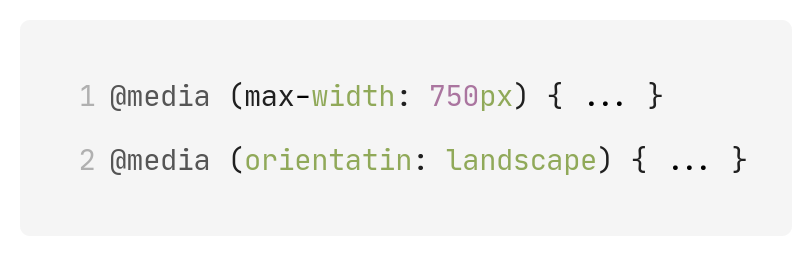
\includegraphics[width=0.6\textwidth]{assets/website2.png}
    \caption{Exemple de \textit{media queries} en CSS.}
    \label{fig:website2}
\end{figure}

Pour réaliser cette amélioration, nous avons utilisé les \textit{media queries} de CSS pour adapter le site web à différentes tailles d'écran.
La Figure \ref*{fig:website2} montre un exemple utilisant cette fonctionnalités du langage CSS.
La première ligne définit le style lorsque la largeur de l'écran est inférieure à 750 pixels, tandis que la deuxième ligne définit le style pour les orientations paysage.



\newpage
\section{Conclusion}
% Written by Louise Fussien

% This file CAN NOT be compiled on its own
% It is included by ../Book_of_Specifications.tex

\subsection{Récapitulatif}

Au terme de notre année académique à l'EPITA, nous sommes fiers de présenter les résultats de notre projet "Lands of Azerith".
Ce projet a été une aventure marquée par des défis techniques, des adaptations organisationnelles, et des innovations créatives.
Nous avons entrepris de développer un jeu vidéo immersif qui non seulement nous a permis de mettre en pratique nos compétences en programmation et en design de jeux,
mais qui a aussi été un véritable terrain d'apprentissage en gestion de projet et en collaboration d'équipe.
\\

Notre projet a commencé avec une vision claire : créer un jeu d'aventure où les joueurs peuvent explorer un monde riche et interactif,
incarner des héros diversifiés, et participer à des quêtes palpitantes. L'acte 1 du jeu, centré sur le village d'Emberwood et ses environs,
a été le cœur de notre développement. Nous avons intégré des mécanismes variés tels que le choix de classes de personnages, la gestion des équipements,
l'utilisation des éléments, et un système de commerce en ville. Chaque étape du jeu a été soigneusement conçue pour offrir une expérience de jeu captivante et fluide.
\\

Le choix de Godot Engine comme moteur de jeu a été déterminant. Godot nous a offert une flexibilité et une puissance adaptées à nos besoins,
sans les contraintes financières des moteurs propriétaires. Nous avons pu exploiter ses capacités pour créer des environnements détaillés et
des mécaniques de jeu complexes. La gestion de version via GitHub a été essentielle pour coordonner nos efforts, permettant une collaboration
efficace malgré les défis liés aux départs de membres et à l'intégration de nouveaux.
\\

La dynamique de notre équipe a connu plusieurs bouleversements.
Le départ d'Alexandre Cohen et de Mohamed Aziz ben Amor a été compensé par l'arrivée de Louise Fussien, qui a apporté une nouvelle énergie et des compétences cruciales. L'utilisation de Discord pour la communication instantanée et des réunions en personne à EPITA a renforcé notre cohésion et notre capacité à résoudre les problèmes rapidement.
La répartition des tâches a été ajustée pour tirer le meilleur parti des compétences de chaque membre, garantissant une progression constante malgré les obstacles.
\\

Partie technique recap

L'aspect visuel et sonore de "Lands of Azerith" a été élaboré avec soin pour immerger les joueurs dans notre univers.
Nous avons puisé notre inspiration dans diverses sources pour créer un design original et attrayant.
L'intégration du son, des effets visuels, et une interface utilisateur intuitive ont été des éléments clés pour enrichir l'expérience de jeu.
Le site web du projet a également été développé pour offrir une vitrine de notre travail, facilitant l'accès à des informations sur le jeu et son développement.
\\

Les défis que nous avons rencontrés, notamment les délais imprévus et les changements d'équipe, ont été surmontés grâce à une planification rigoureuse
et une flexibilité dans notre approche. Nous avons appris à nous adapter rapidement, à redistribuer les responsabilités, et à maintenir notre engagement
envers la qualité du projet. Chaque itération de notre cahier technique a été une occasion de réévaluer et d'améliorer notre travail, assurant que nous
restions alignés sur nos objectifs initiaux tout en intégrant de nouvelles idées et solutions.
\\

\subsection{Remerciements}

Nous tenons à exprimer notre gratitude envers tous ceux qui nous ont soutenus tout au long de ce projet.
Nos professeurs et encadrants à l'EPITA ont été des sources inestimables de conseils et de motivation.
Nous remercions également nos familles et amis pour leur soutien moral et leur patience durant les périodes intenses de développement.
\\

Enfin, nous reconnaissons l'importance des ressources open-source et des communautés de développeurs qui ont contribué indirectement à la réussite de notre projet.
Nous sommes profondément reconnaissants envers ces contributeurs qui ont généreusement partagé leurs connaissances, leurs outils et leur expertise.
Leur contribution a été essentielle pour nous permettre d'aller plus loin dans notre développement et d'atteindre nos objectifs ambitieux.
\\

La richesse des ressources open-source disponibles nous a permis d'accéder à des bibliothèques de code, des frameworks et des outils puissants qui ont grandement facilité notre travail.
Nous avons pu bénéficier de solutions éprouvées et de bonnes pratiques établies par la communauté des développeurs, ce qui nous a fait gagner un temps précieux et nous a évité de réinventer la roue.
\\

De plus, les communautés de développeurs ont été une source inépuisable de soutien et d'inspiration.
Nous avons pu poser des questions, partager nos idées et obtenir des conseils précieux de personnes passionnées et expérimentées.
Leur expertise et leur volonté de partager leurs connaissances ont été une véritable bouffée d'air frais dans notre parcours de développement.
\\

Nous tenons également à souligner l'importance des forums de discussion, des plateformes de partage de code et des sites de documentation en ligne.
Ces ressources ont été des sources inestimables d'informations techniques, de tutoriels détaillés et de réponses à nos problèmes spécifiques.
Grâce à ces plateformes, nous avons pu surmonter des obstacles techniques, acquérir de nouvelles compétences et élargir notre compréhension du développement de jeux vidéo.
\\

Enfin, nous voulons exprimer notre gratitude envers les développeurs qui ont créé et maintenu les outils open-source que nous avons utilisés. Leur travail acharné, leur dévouement et leur passion ont contribué à la qualité et à la fiabilité de ces outils.
Nous sommes conscients que sans leur contribution, notre projet aurait été beaucoup plus difficile à réaliser.
\\

En conclusion, nous reconnaissons l'importance des ressources open-source et des communautés de développeurs dans notre parcours de développement.
Nous sommes profondément reconnaissants envers tous ceux qui ont contribué indirectement à notre projet, que ce soit par le partage de code, la réponse à des questions techniques, ou l'inspiration créative.
\\

Le développement de "Lands of Azerith" ne s'arrête pas à l'acte 1.
Nous envisageons de poursuivre notre travail en développant les actes suivants, en enrichissant l'histoire et les mécaniques de jeu.
Les retours des utilisateurs seront essentiels pour guider nos améliorations et expansions futures.
Notre expérience de cette année nous a équipé des compétences et de la confiance nécessaires pour aborder ces défis avec enthousiasme et détermination.
\\

En conclusion, "Lands of Azerith" est bien plus qu'un simple projet académique.
C'est une réalisation collective qui témoigne de notre passion pour le développement de jeux vidéo, notre capacité à collaborer efficacement, et notre résilience face aux défis.
Nous espérons que ce jeu apportera autant de plaisir aux joueurs qu'il nous en a apporté lors de sa création.
Merci à tous ceux qui ont rendu cette aventure possible.


\section{Annexe}

% Logo of the company
\centering
\vspace*{1.8cm}

\includegraphics[width=3cm]{assets/logo.png}

% Day and time of the last update
\vspace*{1cm}
Last updated on \today{} at \currenttime.

\end{document}
